\documentclass[11pt,letterpaper]{article}

\usepackage{graphicx}
\usepackage[margin=0.90in]{geometry}
\usepackage[T1]{fontenc}
\usepackage[utf8]{inputenc}
\usepackage{authblk}
\usepackage{fancyhdr}
\usepackage{lastpage}
\usepackage[parfill]{parskip}
\usepackage{subcaption}

\pagestyle{fancyplain}
\fancyhf{}
\fancyfoot[R]{\footnotesize Page \thepage\ of \pageref{LastPage}}

\renewcommand{\headrulewidth}{0.0pt} % No header rule
\renewcommand{\footrulewidth}{0.4pt} % Thin footer rule

\begin{document}

\title{Virtual Actor Space for On Demand Distributed Computation}
\author[1]{Benjamin Bengfort}
\author[2]{Allen Leis}
\author[1]{Konstantinos Xirogiannopoulos}
\affil[ ]{Department of Computer Science}
\affil[ ]{University of Maryland}
\affil[1]{\textit{\{bengfort,kostasx\}@cs.umd.edu}}
\affil[2]{\textit{aleis@umd.edu}}

\date{October 21, 2015}

\maketitle
\section*{Introduction}

In order to handle high volume, high velocity computations from sensors, web logs, and other timely data sources a parallel, distributed form of computation is required. In fact, the widespread adoption of distributed computing frameworks and tools has made cluster computing the default, general method of high performance data processing. These frameworks have done much to abstract the details of parallelism and distributed computing away from the developer, thus allowing for a wider community of developers and scientists to take advantage of distributed tool kits.

For streaming data in particular, tools like Spark Streaming \cite{zaharia2012discretized}, Storm \cite{toshniwal2014storm}, and Google DataFlow \cite{akidau2015dataflow} allow the developer to specify a ``data flow'' model of analysis described as a directed graph whose nodes represent a single computation and whose edges represent data transmission of input and output values. Describing computation this way is simple, adaptable, and when mapped to a distributed topology, scalable. However, this model does not allow nodes to communicate, nor provide any flexibility in the computational topology for error handling, transactional guarantees, consistency, or persistence.

Recently, the ``actor model'' \cite{hewitt1973universal} of distributed computation has been re-emerging as an abstraction that does allow for flexible communication between computing nodes. Modern concurrency frameworks such as Akka (formerly Scala Actors) \cite{karmani2009actor} and Erlang Actors \cite{vinoski2007concurrency} expose a high level primitive called an ``actor'' such that everything in the system is an actor that does not share its state, allowing for easy, under-the-hood parallelism. However, a programming model alone is not enough in a distributed context -- the tools mentioned above also provide an execution and job management context. Orleans \cite{bernstein_orleans_2015} gives developers a virtual ``actor space'' that is analogous to virtual memory. Developers can then invoke any actor in the system regardless if it's present in memory; this allows Orleans to address problems such as actor placement, load balancing, deactivation of unused actors, and even recover from actor failure.

We intend to take the ``virtual actor space'' concept one step farther and create a generalized architecture for actor-based data processing. The generalized architecture will provide a stage for simultaneous actor computation, will facilitate actor management and communication, and will provide actor resources in an on-demand fashion. By providing an ``actor-as-a-service'' framework for development, programmers will only have to specify what actors are and how they communicate. Moreover, we intend to demonstrate that this model improves upon data flow computation by providing stateful, dynamically allocated resources and by allowing for inter-actor communication.

%We intend to show that our framework is simpler to develop on, and has more opportunities for load balancing and error handling than current frameworks.


% The widespread adoption of distributed computing frameworks and tools has led to a ``data flow'' model of data analysis. Data flows are described as directed graphs whose nodes represent a single computation and whose edges represent data transmission of input and output values.  Another model of computation that has been re-emerging is what is known as the ``actor model", which focuses on defining an intuitive layer of abstraction that allows users to easily reason about and deal with a lot of difficult problems in concurrent computation systems.
%
% The traditional actor model~, has been implemented in modern frameworks such as Akka and Erlang/lixir revolves around the idea that in order to make sense of distributed computing, we must abstract each entity into a high level primitive called an ``actor" so that everything on the system is an actor. Actors embody all essential elements of computation namely : (1) processing, (2) state, and (3) communication. In this actor world, computation happens by actors communicating with each-other through messages, processing information and altering their state.
%
% As described above, apart from providing an intuitive abstraction, the power of the actor model is derived from the fact that computation is not steered towards only one direction like in the ``data flow" model. The data flow model requires computation to flow from a set of computation nodes towards other ones in a single unified stream through a Directed Acyclic Graph whereas in the actor model, actors are free to exchange messages freely with eachother throughout the system with no restrictions on the direction in which the data is flowing because actors unlike data flow spouts, are stateful.

\section*{Proposal}

\begin{figure}[t]
	\centering
    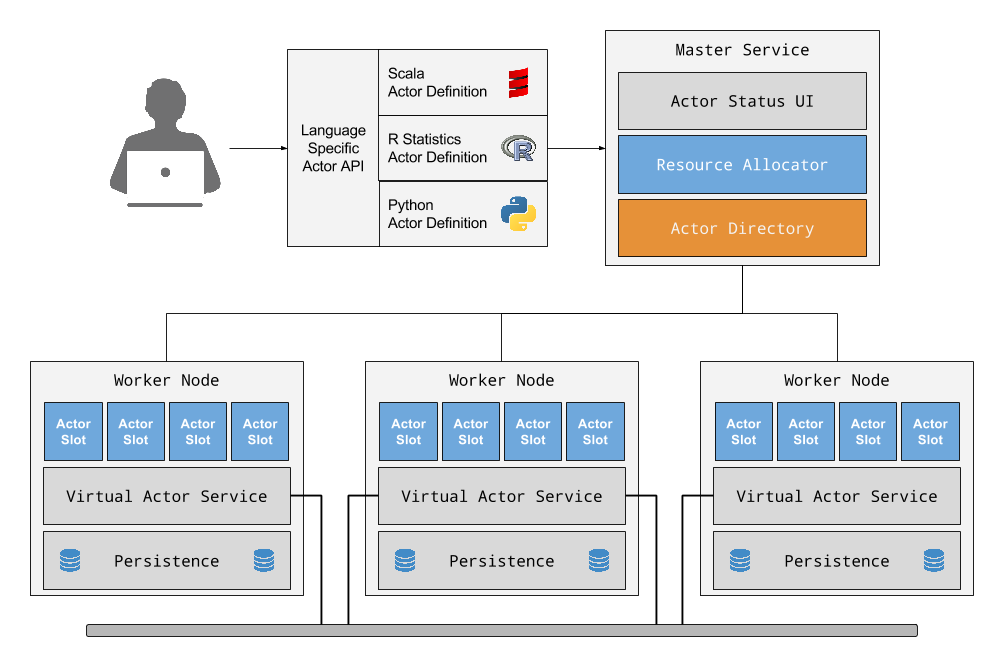
\includegraphics[width=0.8\textwidth]{figures/architecture.png}
    \caption{\textsf{Architecture of a virtual actor space that generalizes on-demand distributed computation. A director controls job submission and resource allocation, while worker nodes manage Actor instances. Actors communicate with each other and have a state which persists to disk and is reloaded upon re-instantiation.}}
    \label{fig:architecture}
\end{figure}

An Actor is responsible for all essential elements of a single computation including (1) processing, (2) state, and (3) communication. An analytical job therefore takes the form of a series of actors that accept incoming data, perform processing, and communicate with each other, thereby altering the state of computational space. Because each Actor has its own independent state, an Actor framework or stage can easily instantiate Actors on a variety of nodes and facilitate communication between them, thus abstracting much of the low level details away from the developer.

We propose to develop a proof of concept Actor framework to show that this abstraction is beneficial to developers and will facilitate computations that do require multiple communication streams. A simple, proposed architecture is shown in Figure \ref{fig:architecture}. This basic architecture will allow us to develop towards research grade projects including developing an Actor consistency model. In this project, we intend to show the benefits of an actor model by adapting the following applications to Actor space:

\begin{enumerate}
	\item Timely email analytics data flow
	\item Domain decomposition (Game of Life)
	\item Book Recommendation using Non-Negative Matrix Factorization
\end{enumerate}

We will measure the performance of the Actor framework including the ability to handle multiple, streaming applications simultaneously as well as its ability to persist and recover from failure. We will also show through a simple user study the benefits and ease of use of the Actor model.

\bibliographystyle{plain}
\bibliography{papers}

\end{document}
